% !TEX program = lualatex
\documentclass[12pt,a4paper]{article}
\usepackage{graphicx}
\usepackage{fontspec}
\setmonofont{Latin Modern Mono}
\usepackage{xcolor}
\usepackage{listings}
\usepackage{geometry}
\usepackage{fancyhdr}
\usepackage{hyperref}
\usepackage{booktabs} 
\usepackage{float}    
\usepackage{amsmath}

% =======================================================
%  USER CONFIGURATION (EDIT VARIABLES HERE)
% =======================================================
\newcommand{\labNo}{Lab 5}
\newcommand{\labTopic}{The Server Room Heist: Joins and Aggregates}
\newcommand{\courseCode}{CSE 4308}
\newcommand{\courseTitleShort}{DBMS Lab}
\newcommand{\courseTitleLong}{DATABASE MANAGEMENT SYSTEMS LAB}
\newcommand{\instructorName}{Samnun Azfar, Jr. Lecturer, CSE\\ Samia Nawsheen, Jr. Lecturer, CSE}
\newcommand{\academicYear}{AY25-26}
% =======================================================

\geometry{margin=1in}

% -
% Header and Footer Configuration
% -
\pagestyle{fancy}
\fancyhf{}
\lhead{\labNo}                        % Uses variable
\rhead{\courseCode: \courseTitleShort} % Uses variables

% Centered footer with page number
\cfoot{\thepage}
% Ensure header/footer width matches text block
\setlength{\headwidth}{\textwidth}

% -
% Code Listing Style
% -
\definecolor{codegreen}{rgb}{0,0.6,0}
\definecolor{codegray}{rgb}{0.5,0.5,0.5}
\definecolor{codepurple}{rgb}{0.58,0,0.82}
\definecolor{backcolour}{rgb}{0.95,0.95,0.92}

\lstdefinestyle{mystyle}{
    backgroundcolor=\color{backcolour},
    commentstyle=\color{codegreen},
    keywordstyle=\color{magenta},
    numberstyle=\tiny\color{codegray},
    stringstyle=\color{codepurple},
    basicstyle=\ttfamily\footnotesize,
    breaklines=true,
    captionpos=b,
    keepspaces=true,
    numbers=left,
    numbersep=5pt,
    tabsize=2,
    frame=single,
    numbers=none,
    columns=fullflexible,
    showspaces=false,
    showstringspaces=false,
    showtabs=false,
    language=SQL
}

\lstset{style=mystyle}

% Images: found next to this file (local compile_labs.sh) or via the
% lab folder when compiled from the project root (Overleaf).
\graphicspath{{lab_05_joins_aggregate_functions_group/}}

\begin{document}

% --
% TITLE PAGE
% --
\begin{titlepage}
    \centering
    \vspace*{2\baselineskip}

    \rule{14cm}{2pt}\vspace*{-0.8\baselineskip}\vspace*{1.5pt}
    \rule{14cm}{0.5pt}\vspace{2\baselineskip}

    {\Huge\bfseries\scshape \labNo\par} % Uses variable
    \vspace{3mm}
    {\Large \labTopic} % Uses variable
    \vspace{3mm}

    \rule{14cm}{0.5pt}\vspace*{-0.7\baselineskip}\vspace{2.5pt}
    \rule{14cm}{2pt}

    \vspace{2\baselineskip}

    {\Large\bfseries \courseCode\par} % Uses variable
    \vspace{1\baselineskip}
    {\large \courseTitleLong\par} % Uses variable

    \vfill
    {\normalsize Prepared by:\\ \instructorName\par} % Uses variable
    {\normalsize Academic Year: \academicYear\par} % Uses variable
\end{titlepage}

\newpage
\tableofcontents
\newpage
\section*{Lab Workflow}



\textit{Repeat this subsection for every single lab.}

\begin{enumerate}
\item Connect to the internet by running nmtui in terminal, add a dsl connection, then go back and activate that dsl connection. Make sure that your net id is not being used in any other pc or router, if you face any issue, use any other net id from your friends which is not being used.

\item Download all the files posted in the google classroom.

\item Disconnect from the \textbf{dsl} connection via nmtui, connect to the ethernet/wired connection via nmtui. If no such connection exists, create an \textbf{ethernet} connection  and then activate.

    \item \textbf{Create Your Role and Database}

Inside the PostgreSQL shell, create your own role (user) and database.

1. In the Linux terminal:
\begin{lstlisting}[language=bash]
psql
\end{lstlisting}

Expected prompt:
\begin{lstlisting}
cse=#
\end{lstlisting}

2. Create Your Role and Database

Copy and run the following commands inside PostgreSQL:
\begin{lstlisting}[language=SQL]
-- 1. Terminate existing database connections
SELECT pg_terminate_backend(pid)
FROM pg_stat_activity
WHERE datname = 'cse4308_12345'
  AND pid <> pg_backend_pid();

-- 2. Remove existing database
DROP DATABASE IF EXISTS cse4308_12345;

-- 3. Remove existing role
DROP ROLE IF EXISTS student_12345;

-- 4. Create role
CREATE ROLE student_12345 LOGIN;

-- 5. Set password
ALTER ROLE student_12345
WITH PASSWORD 'student12345';

-- 6. Create database
CREATE DATABASE cse4308_12345
OWNER student_12345;

-- 7. Grant privileges
GRANT ALL PRIVILEGES
ON DATABASE cse4308_12345
TO student_12345;
\end{lstlisting}

3. Exit PostgreSQL:

   \begin{lstlisting}[language=SQL]
   \q
   \end{lstlisting}

\item \textbf{Connect Using Your Newly Created User}

1. Connect to Your Database:

   Use the following command to log in as the \texttt{student\_12345} user:

   \begin{lstlisting}[language=SQL]
   psql -h localhost -U student_12345 -d cse4308_12345
   \end{lstlisting}

2. Verify the Connection:

   Verify that you are connected to the correct database with the following command:

   \begin{lstlisting}[language=SQL]
   \conninfo
   \end{lstlisting}

   Expected output:

   \begin{lstlisting}
   Database: cse4308_12345, User: student_12345
   \end{lstlisting}

3. Exit PostgreSQL:

   \begin{lstlisting}[language=SQL]
   \q
   \end{lstlisting}

\item \textbf{Load the Lab SQL File (MUST be run outside psql)}

Load the SQL file that sets up the tables and inserts initial data.

1. Load the SQL File:

   Run the following command to load the lab SQL file:

   \begin{lstlisting}[language=SQL]
   psql -h localhost -U student_12345 -d cse4308_12345 -f /home/cse/Downloads/lab_05_setup.sql
   \end{lstlisting}

   This will:
   - Drop old tables (if they exist).
   - Create new tables.
   - Insert initial rows of data.

\item \textbf{Reconnect and Verify Tables}

After loading the SQL file, reconnect to PostgreSQL to verify that the tables have been created.

1. Reconnect to Your Database:

   \begin{lstlisting}[language=SQL]
   psql -h localhost -U student_12345 -d cse4308_12345
   \end{lstlisting}

2. Check Tables:

   Verify the tables have been created by listing them:

   \begin{lstlisting}[language=SQL]
   \dt
   \end{lstlisting}

3. View Table Data:

   Verify the data by running the following SQL queries:

   \begin{lstlisting}[language=SQL]
   SELECT * FROM <table_name>;
   \end{lstlisting}

\item Open a text editor and save it in the appropriate submission name format \\ \texttt{fullid\_CSE4308\_L5\_T1.sql}. You will use this text editor to write your solutions, make sure to save it after writing each solution. The structure of this file will be:
\begin{lstlisting}[language=SQL]
-- Task 1
INSERT INTO students (student_id, name, major, gpa)
VALUES (104, 'David', 'ME', 3.60);
--Task 2
SELECT name, gpa FROM students WHERE major = 'CSE';
\end{lstlisting}
\end{enumerate}
\newpage

\newpage
\section{Investigative Database Schema}

At University X, the Server Room houses sensitive exam questions and research data. On December 7, 2026, a security breach occurred. Someone physically entered the Server Room and deployed a script to leak data. The physical security logs, cafeteria receipts, and library records are the only evidence left behind. You are the Lead Database Detective hired to identify the culprit among the staff and students. You must do the following to solve the tasks:
\begin{enumerate}
    \item Intelligence Gathering
    \item Connecting the Dots based on gathered info. Cross-reference the Suspects with the Access Logs and Locations.
    \item Look for anomalies. Who has never borrowed a book? Who has never ordered food? Who has no access logs at all?
    \item Behavioral Analysis among the suspects
    \item Follow this trail of breadcrumbs and catch the hacker before they wipe the database logs!
\end{enumerate}

\noindent To solve the crime, you must understand the relationships between the entities on campus. We will use the following three sample tables for the lecture examples: \textbf{suspects}, \textbf{locations}, and \textbf{access\_logs}.

\subsection*{Table 1: suspects}
\begin{table}[H]
\centering
\begin{tabular}{@{}lllc@{}}
\toprule
\textbf{suspect\_id} (PK) & \textbf{name} & \textbf{occupation} & \textbf{access\_level} \\ \midrule
1 & Zahid & Exam Controller & 5 \\
2 & Nafis & Student & 1 \\
3 & Tabib & Research Assistant & 4 \\
4 & Sieam & Student & 1 \\ \bottomrule
\end{tabular}
\end{table}

\subsection*{Table 2: locations}
\begin{table}[H]
\centering
\begin{tabular}{@{}lllc@{}}
\toprule
\textbf{location\_id} (PK) & \textbf{location\_name} & \textbf{floor\_number} \\ \midrule
101 & Server Room & 3 \\
102 & North Canteen & 1 \\
103 & Library & 2 \\ \bottomrule
\end{tabular}
\end{table}

\subsection*{Table 3: access\_logs}
\begin{table}[H]
\centering
\begin{tabular}{@{}llllc@{}}
\toprule
\textbf{log\_id} (PK) & \textbf{suspect\_id} (FK) & \textbf{location\_id} (FK) & \textbf{entry\_time} \\ \midrule
901 & 1 & 101 & 14:00 \\
902 & 2 & 102 & 14:10 \\
903 & 1 & 102 & 15:00 \\
904 & 3 & 101 & 09:00 \\ \bottomrule
\end{tabular}
\end{table}

\subsection*{Database Setup Code (For Lecture Demo)}
This is just to understand the structure. The sql for your task is different.

\begin{lstlisting}
CREATE TABLE suspects (
    suspect_id SERIAL PRIMARY KEY,
    name VARCHAR(50),
    occupation VARCHAR(50),
    access_level INT
);

CREATE TABLE locations (
    location_id SERIAL PRIMARY KEY,
    location_name VARCHAR(100),
    floor_number INT
);

CREATE TABLE access_logs (
    log_id SERIAL PRIMARY KEY,
    suspect_id INT REFERENCES suspects(suspect_id),
    location_id INT REFERENCES locations(location_id),
    entry_time TIMESTAMP
);
\end{lstlisting}

\begin{figure}[h]
    \centering
    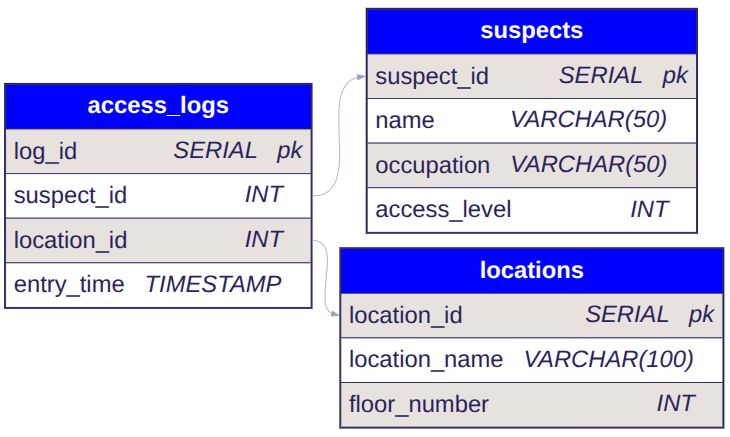
\includegraphics[width=0.8\linewidth]{lab_05_figure.png}
\end{figure}
\newpage
\section{Technique 1: Connecting Evidence (SQL Joins)}
Detectives use Joins to connect a person (Suspect) to a place (Location) via evidence (Logs).

\subsection{INNER JOIN (Confirmed Presence)}
The \texttt{INNER JOIN} returns records only when there is a match in \textbf{both} tables. It answers: "Who definitely swiped their card?"

\textbf{Query:} Show Suspect Names and the Location IDs they visited.
\begin{lstlisting}
SELECT S.name, A.location_id, A.entry_time
FROM suspects S
INNER JOIN access_logs A ON S.suspect_id = A.suspect_id;
\end{lstlisting}

\textbf{Result:}
\textit{Note: Sieam (ID 4) is not listed because he has no log entry.}
\begin{table}[H]
\centering
\begin{tabular}{@{}lll@{}}
\toprule
\textbf{name} & \textbf{location\_id} & \textbf{entry\_time} \\ \midrule
Zahid & 101 & 14:00 \\
Nafis & 102 & 14:10 \\
Zahid & 102 & 15:00 \\
Tabib & 101 & 09:00 \\ \bottomrule
\end{tabular}
\end{table}
\subsection{NATURAL JOIN (The Implicit Connection)}
A \texttt{NATURAL JOIN} is a shortcut. It automatically performs an \texttt{INNER JOIN} by looking for columns with the \textbf{same name} and data type in both tables. In our case, both \textbf{suspects} and \textbf{access\_logs} share the column \texttt{suspect\_id}.

\textbf{Query:} Join Suspects and Logs without specifying the \texttt{ON} condition.
\begin{lstlisting}
SELECT name, entry_time
FROM suspects
NATURAL JOIN access_logs;
\end{lstlisting}

\textbf{Result:}
The database automatically detected \texttt{suspect\_id} as the common key.
\begin{table}[H]
\centering
\begin{tabular}{@{}ll@{}}
\toprule
\textbf{name} & \textbf{entry\_time} \\ \midrule
Zahid & 14:00 \\
Nafis & 14:10 \\
Zahid & 15:00 \\
Tabib & 09:00 \\ \bottomrule
\end{tabular}
\end{table}

\textbf{Detective's Warning:} Use this technique with caution! If your tables accidentally share a column name that isn't a foreign key (e.g., both tables have a generic \texttt{comment} or \texttt{created\_at} column), the Natural Join will try to match those as well, leading to incorrect results or empty tables.

\subsection{Joining Three Tables}
To see the \textbf{Location Name} instead of the ID, we join a third table.

\textbf{Query:} Show Suspect Name and Location Name.
\begin{lstlisting}
SELECT S.name, L.location_name
FROM suspects S
JOIN access_logs A ON S.suspect_id = A.suspect_id
JOIN locations L ON A.location_id = L.location_id;
\end{lstlisting}

\newpage
\section{Technique 2: Finding Missing Links}
Sometimes, what is \textbf{missing} is the most important clue.

\subsection{LEFT JOIN}
Returns all records from the left table (Suspects), and matched records from the right (Logs). If a suspect has no logs, they appear with NULLs.

\textbf{Query:} List all suspects and their visit times. Include those who did not visit anywhere.
\begin{lstlisting}
SELECT S.name, A.entry_time
FROM suspects S
LEFT JOIN access_logs A ON S.suspect_id = A.suspect_id;
\end{lstlisting}

\textbf{Result:}
\textit{Sieam has NULL entry\_time, meaning he left no digital footprint.}
\begin{table}[H]
\centering
\begin{tabular}{@{}ll@{}}
\toprule
\textbf{name} & \textbf{entry\_time} \\ \midrule
Zahid & 14:00 \\
Zahid & 15:00 \\
Nafis & 14:10 \\
Tabib & 09:00 \\
Sieam & \textit{NULL} \\ \bottomrule
\end{tabular}
\end{table}

\subsection{RIGHT JOIN}
Returns all records from the right table. Useful to find logs that don't match a known suspect (e.g., a corrupted ID).

\textbf{Query:} Show all Logs and the associated Suspect Name.
\begin{lstlisting}
SELECT S.name, A.entry_time
FROM suspects S
RIGHT JOIN access_logs A ON S.suspect_id = A.suspect_id;
\end{lstlisting}

\section{Technique 3: Profiling (Aggregates)}

\subsection{COUNT, SUM, AVG, MAX}
\textbf{Query:} Get statistics on the suspects.
\begin{lstlisting}
SELECT 
    COUNT(*) AS total_suspects,
    MAX(access_level) AS highest_clearance,
    AVG(access_level) AS avg_clearance
FROM suspects;
\end{lstlisting}

\textbf{Result:}
\begin{table}[H]
\centering
\begin{tabular}{@{}lll@{}}
\toprule
\textbf{total\_suspects} & \textbf{highest\_clearance} & \textbf{avg\_clearance} \\ \midrule
4 & 5 & 2.75 \\ \bottomrule
\end{tabular}
\end{table}

\section{Technique 4: Grouping Suspects (GROUP BY)}

\subsection{GROUP BY with Aggregate}
\textbf{Query:} Count how many times \textbf{each} suspect swiped their card.
\begin{lstlisting}
SELECT suspect_id, COUNT(*) AS visit_count
FROM access_logs
GROUP BY suspect_id;
\end{lstlisting}

\textbf{Result:}
\begin{table}[H]
\centering
\begin{tabular}{@{}ll@{}}
\toprule
\textbf{suspect\_id} & \textbf{visit\_count} \\ \midrule
1 (Zahid) & 2 \\
2 (Nafis) & 1 \\
3 (Tabib) & 1 \\ \bottomrule
\end{tabular}
\end{table}

\subsection{GROUP BY with JOIN (Readable Report)}
\textbf{Query:} Count visits per Location Name.
\begin{lstlisting}
SELECT L.location_name, COUNT(A.log_id) AS total_visits
FROM locations L
JOIN access_logs A ON L.location_id = A.location_id
GROUP BY L.location_name;
\end{lstlisting}

\textbf{Result:}
\begin{table}[H]
\centering
\begin{tabular}{@{}ll@{}}
\toprule
\textbf{location\_name} & \textbf{total\_visits} \\ \midrule
Server Room & 2 \\
North Canteen & 2 \\ \bottomrule
\end{tabular}
\end{table}

\section{Technique 5: Narrowing the List (HAVING)}
The \texttt{HAVING} clause filters groups \textbf{after} the aggregation. It is essential for finding "suspiciously high" activity.

\subsection{HAVING Clause}
\textbf{Query:} Find suspects who visited locations \textbf{more than 1 time}.
\begin{lstlisting}
SELECT suspect_id, COUNT(*) AS visit_count
FROM access_logs
GROUP BY suspect_id
HAVING COUNT(*) > 1;
\end{lstlisting}

\textbf{Result:}
\textit{Only Zahid is listed.}
\begin{table}[H]
\centering
\begin{tabular}{@{}ll@{}}
\toprule
\textbf{suspect\_id} & \textbf{visit\_count} \\ \midrule
1 & 2 \\ \bottomrule
\end{tabular}
\end{table}

\newpage

\section{Lab Tasks}

\begin{figure}[h]
    \centering
    % Left Bottom Right Top
    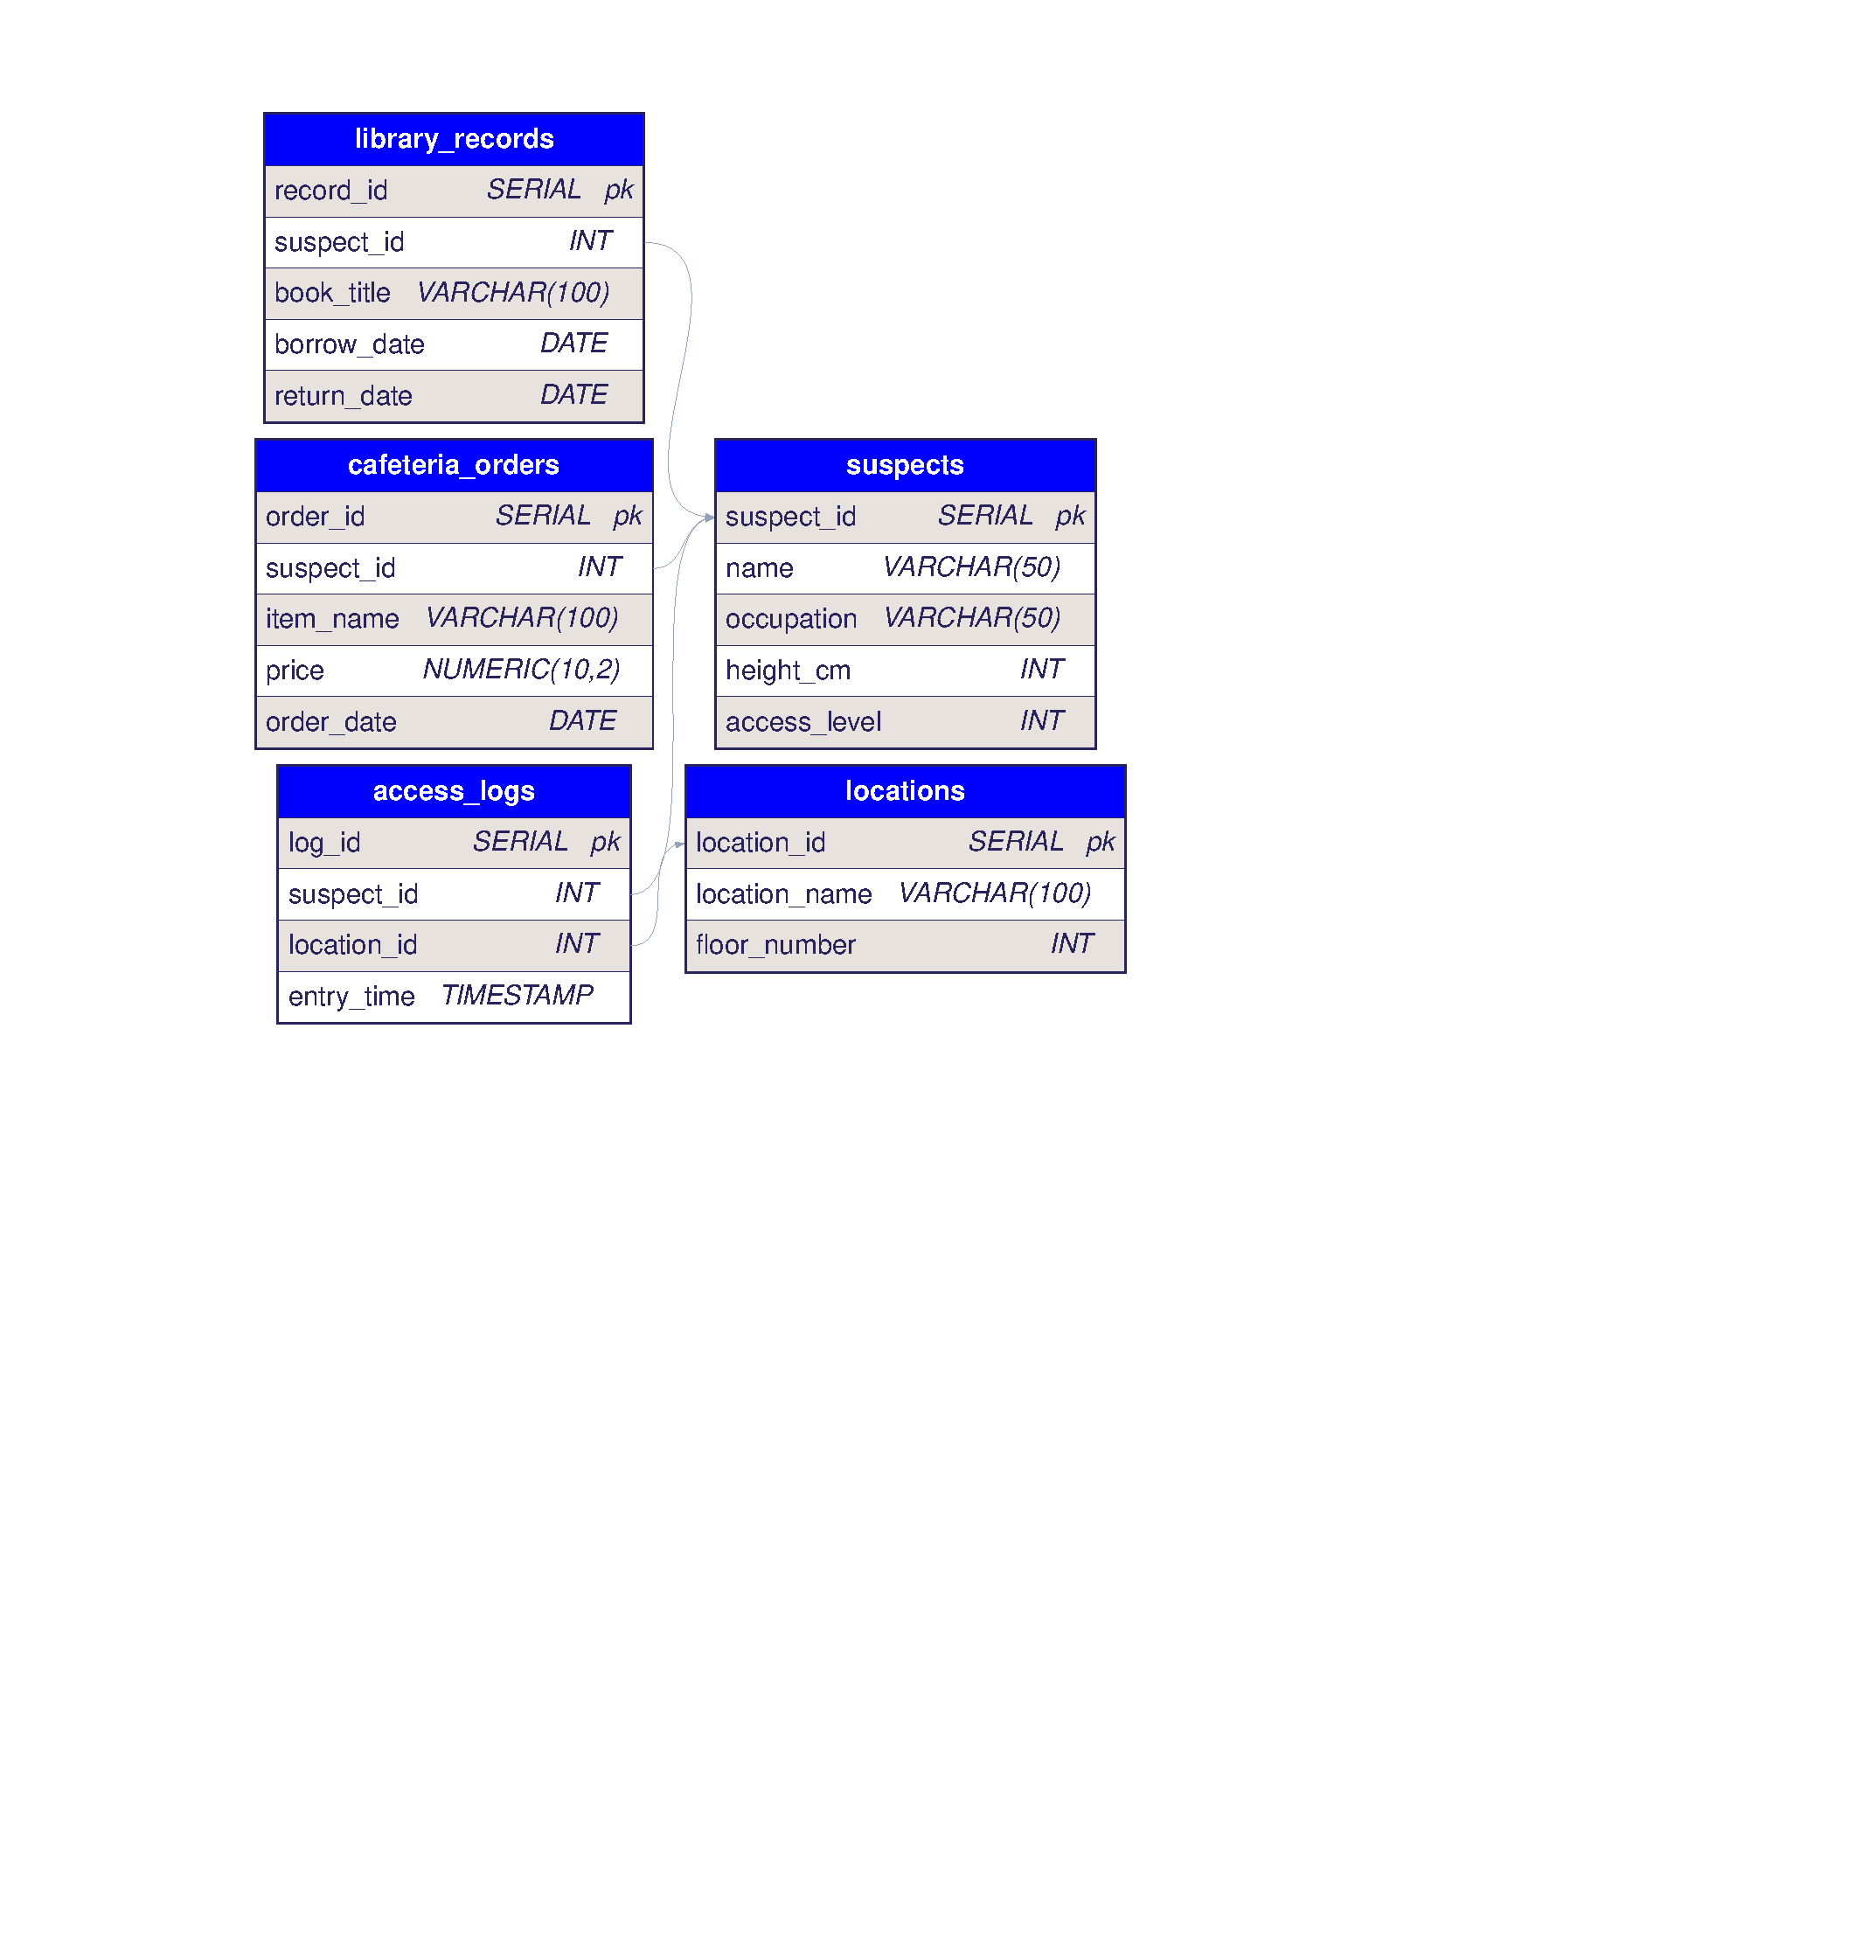
\includegraphics[trim={0cm 20cm 10cm 0cm}, clip, width=0.8\textwidth]{lab_05_erd.pdf}
\end{figure}

\begin{enumerate}
% ==================================================================
% PHASE 1: INTELLIGENCE GATHERING (Basic SELECT / WHERE)
% ==================================================================

    % \item Retrieve the names and occupations of all people in the \texttt{suspects} table who have an \texttt{access\_level} greater than 3.
    % Solution:
    % SELECT name, occupation FROM suspects WHERE access_level > 3;

    % \item List all cafeteria orders where the price is greater than 100 Taka. Show the item name and price.
    % Solution:
    % SELECT item_name, price FROM cafeteria_orders WHERE price > 100;

    % \item Find the location names that are situated on the 1st Floor (from the \texttt{locations} table).
    % Solution:
    % SELECT location_name FROM locations WHERE floor_number = 1;

    \item List the names of all suspects who are taller than 175 cm.
    % Solution:
    % SELECT name FROM suspects WHERE height_cm > 175;

    % \item Show the titles of all books borrowed from the library that have NOT been returned yet (where \texttt{return\_date} is NULL).
    % Solution:
    % SELECT book_title FROM library_records WHERE return_date IS NULL;

    % \item List the details of all access logs that occurred on '2024-12-01'.
    % Solution:
    % SELECT * FROM access_logs WHERE entry_time::DATE = '2024-12-01';

% ==================================================================
% PHASE 2: CONNECTING THE DOTS (INNER JOIN)
% ==================================================================
    % \item Display the \textbf{Suspect Name} and the \textbf{Location Name} they visited by joining \texttt{suspects}, \texttt{access\_logs}, and \texttt{locations}.
    % Solution:
    % SELECT s.name, l.location_name
    % FROM suspects s
    % JOIN access_logs a ON s.suspect_id = a.suspect_id
    % JOIN locations l ON a.location_id = l.location_id;

    % \item Find out what items each person bought. Display \textbf{Suspect Name} and \textbf{Item Name} by joining \texttt{suspects} and \texttt{cafeteria\_orders}.
    % Solution:
    % SELECT s.name, c.item_name
    % FROM suspects s
    % JOIN cafeteria_orders c ON s.suspect_id = c.suspect_id;

    % \item Show a list of \textbf{Occupations} and the \textbf{Books} they are reading. Join \texttt{suspects} and \texttt{library\_records}.
    % Solution:
    % SELECT s.occupation, l.book_title
    % FROM suspects s
    % JOIN library_records l ON s.suspect_id = l.suspect_id;

    \item List the \textbf{Location Name} and the \textbf{Entry Time} for anyone who is a \texttt{'Student'}.
    % Solution:
    % SELECT l.location_name, a.entry_time
    % FROM access_logs a
    % JOIN locations l ON a.location_id = l.location_id
    % JOIN suspects s ON a.suspect_id = s.suspect_id
    % WHERE s.occupation = 'Student';

    % \item Find the total price of items bought by 'Exam Controllers'. Display \textbf{Name}, \textbf{Item}, and \textbf{Price}.
    % Solution:
    % SELECT s.name, c.item_name, c.price
    % FROM suspects s
    % JOIN cafeteria_orders c ON s.suspect_id = c.suspect_id
    % WHERE s.occupation = 'Exam Controller';

    % \item List the \textbf{Names} of suspects who visited the 'Server Room'. You must join tables to filter by location name 'Server Room'.
    % Solution:
    % SELECT s.name
    % FROM suspects s
    % JOIN access_logs a ON s.suspect_id = a.suspect_id
    % JOIN locations l ON a.location_id = l.location_id
    % WHERE l.location_name = 'Server Room';

% ==================================================================
% PHASE 3: FINDING THE GAPS (LEFT / RIGHT JOIN)
% ==================================================================
% Note: These queries test if students can find missing data (NULLs)
    % \item List all suspect names and their borrowed book titles. You MUST include suspects who have \textbf{never} borrowed a book (use LEFT JOIN).
    % Solution:
    % SELECT s.name, l.book_title
    % FROM suspects s
    % LEFT JOIN library_records l ON s.suspect_id = l.suspect_id;

    % \item List all suspect names and their cafeteria orders. Include suspects who have \textbf{not ordered} anything (result should show NULL for item).
    % Solution:
    % SELECT s.name, c.item_name
    % FROM suspects s
    % LEFT JOIN cafeteria_orders c ON s.suspect_id = c.suspect_id;

    % \item List all Location names and the entry times of people visiting them. Include locations that have \textbf{never} been visited.
    % Solution:
    % SELECT l.location_name, a.entry_time
    % FROM locations l
    % LEFT JOIN access_logs a ON l.location_id = a.location_id;

    \item Perform a RIGHT JOIN between \texttt{suspects} and \texttt{access\_logs} to list all logs and the associated suspect name.
    % Solution:
    % SELECT s.name, a.*
    % FROM suspects s
    % RIGHT JOIN access_logs a ON s.suspect_id = a.suspect_id;

    % \item List all Suspect Names and all Book Titles using a FULL OUTER JOIN. This shows everyone (readers and non-readers) and potentially unassigned books.
    % Solution:
    % SELECT s.name, l.book_title
    % FROM suspects s
    % FULL OUTER JOIN library_records l ON s.suspect_id = l.suspect_id;

    % \item List all 'System Admin' or 'Lab Attendant' names and their orders. Include those who bought nothing.
    % Solution:
    % SELECT s.name, c.item_name
    % FROM suspects s
    % LEFT JOIN cafeteria_orders c ON s.suspect_id = c.suspect_id
    % WHERE s.occupation IN ('System Admin', 'Lab Attendant');

% ==================================================================
% PHASE 4: BEHAVIORAL ANALYSIS (AGGREGATES & GROUP BY)
% ==================================================================
    % \item Calculate the total amount of money (\texttt{SUM}) spent by each suspect. Display \textbf{Suspect Name} and \textbf{Total Spent}.
    % Solution:
    % SELECT s.name, SUM(c.price) AS total_spent
    % FROM suspects s
    % JOIN cafeteria_orders c ON s.suspect_id = c.suspect_id
    % GROUP BY s.name;

    % \item Count how many times each \textbf{Location} was visited. Display Location Name and Visit Count.
    % Solution:
    % SELECT l.location_name, COUNT(a.log_id) AS visit_count
    % FROM locations l
    % JOIN access_logs a ON l.location_id = a.location_id
    % GROUP BY l.location_name;

    % \item Find the average height of suspects grouped by their \textbf{Occupation}.
    % Solution:
    % SELECT occupation, AVG(height_cm)
    % FROM suspects
    % GROUP BY occupation;

    \item Count how many books each suspect has borrowed. Display Name and Book Count.
    % Solution:
    % SELECT s.name, COUNT(l.record_id) AS book_count
    % FROM suspects s
    % JOIN library_records l ON s.suspect_id = l.suspect_id
    % GROUP BY s.name;

    % \item Find the most expensive item purchased (MAX Price) for each suspect.
    % Solution:
    % SELECT s.name, MAX(c.price) AS max_price
    % FROM suspects s
    % JOIN cafeteria_orders c ON s.suspect_id = c.suspect_id
    % GROUP BY s.name;

    % \item Calculate the total number of people with each \textbf{Access Level}. (e.g., Level 5: 2 people).
    % Solution:
    % SELECT access_level, COUNT(*) AS people_count
    % FROM suspects
    % GROUP BY access_level;

% ==================================================================
% PHASE 5: THE FINAL ACCUSATION (HAVING & COMPLEX LOGIC)
% ==================================================================

    % \item Find the names of suspects who have spent \textbf{more than 200 Taka} in total at the cafeteria. (Use HAVING).
    % Solution:
    % SELECT s.name, SUM(c.price)
    % FROM suspects s
    % JOIN cafeteria_orders c ON s.suspect_id = c.suspect_id
    % GROUP BY s.name
    % HAVING SUM(c.price) > 200;

    % \item Find the Location Names that have been visited by \textbf{more than 1 person}.
    % Solution:
    % SELECT l.location_name
    % FROM locations l
    % JOIN access_logs a ON l.location_id = a.location_id
    % GROUP BY l.location_name
    % HAVING COUNT(a.suspect_id) > 1;

    % \item Find the name of the suspect who has borrowed a book with the word 'Hacking' in the title. (Use wildcard \%).
    % Solution:
    % SELECT s.name
    % FROM suspects s
    % JOIN library_records l ON s.suspect_id = l.suspect_id
    % WHERE l.book_title LIKE '%Hacking%';

    \item Find the name of the suspect who entered the \texttt{'Server Room'} AND has an Access Level of 5.
    % Solution:
    % SELECT s.name
    % FROM suspects s
    % JOIN access_logs a ON s.suspect_id = a.suspect_id
    % JOIN locations l ON a.location_id = l.location_id
    % WHERE l.location_name = 'Server Room' AND s.access_level = 5;

    % \item Find the name of the suspect who entered the 'Server Room' between 14:00 and 15:00 on '2024-12-01'.
    % Solution:
    % SELECT s.name
    % FROM suspects s
    % JOIN access_logs a ON s.suspect_id = a.suspect_id
    % JOIN locations l ON a.location_id = l.location_id
    % WHERE l.location_name = 'Server Room'
    % AND a.entry_time BETWEEN '2024-12-01 14:00:00' AND '2024-12-01 15:00:00';

    % \item Combine the clues: Who is an 'Exam Controller', has borrowed a book, and entered the 'Server Room'?
    % Solution:
    % SELECT s.name
    % FROM suspects s
    % JOIN library_records lr ON s.suspect_id = lr.suspect_id
    % JOIN access_logs al ON s.suspect_id = al.suspect_id
    % JOIN locations loc ON al.location_id = loc.location_id
    % WHERE s.occupation = 'Exam Controller'
    % AND loc.location_name = 'Server Room';

\end{enumerate}
\end{document}